\documentclass{article}

\usepackage{amsmath,amssymb}
\usepackage{tikz}
\usepackage{pgfplots}
\usepackage{xcolor}
\usepackage[left=2.1cm,right=3.1cm,bottom=3cm,footskip=0.75cm,headsep=0.5cm]{geometry}
\usepackage{enumerate}
\usepackage{enumitem}
\usepackage{marvosym}
\usepackage{tabularx}

\usepackage{listings}
\definecolor{lightlightgray}{rgb}{0.95,0.95,0.95}
\definecolor{lila}{rgb}{0.8,0,0.8}
\definecolor{mygray}{rgb}{0.5,0.5,0.5}
\definecolor{mygreen}{rgb}{0,0.8,0.26}
\lstdefinestyle{java} {language=java}
\lstset{language=java,
	basicstyle=\ttfamily,
	keywordstyle=\color{lila},
	commentstyle=\color{lightgray},
	stringstyle=\color{mygreen}\ttfamily,
	backgroundcolor=\color{white},
	showstringspaces=false,
	numbers=left,
	numbersep=10pt,
	numberstyle=\color{mygray}\ttfamily,
	identifierstyle=\color{blue},
	xleftmargin=.1\textwidth, 
	%xrightmargin=.1\textwidth,
	escapechar=§,
	breaklines=true,
	postbreak=\mbox{\space}
}

\usepackage[utf8]{inputenc}

\renewcommand*{\arraystretch}{1.4}

\newcolumntype{L}[1]{>{\raggedright\arraybackslash}p{#1}}
\newcolumntype{R}[1]{>{\raggedleft\arraybackslash}p{#1}}
\newcolumntype{C}[1]{>{\centering\let\newline\\\arraybackslash\hspace{0pt}}m{#1}}

\newcommand{\E}{\mathbb{E}}
\DeclareMathOperator{\rk}{rk}
\DeclareMathOperator{\Var}{Var}
\DeclareMathOperator{\Cov}{Cov}

\title{\textbf{Softwaretechnologie, Übung 8}}
\author{\textsc{Henry Haustein}}
\date{}

\begin{document}
	\maketitle
	
	\section*{Aufgabe 1}
	\begin{enumerate}[label=(\alph*)]
		\item Observer
		\item UML-Diagramm
		\begin{center}
			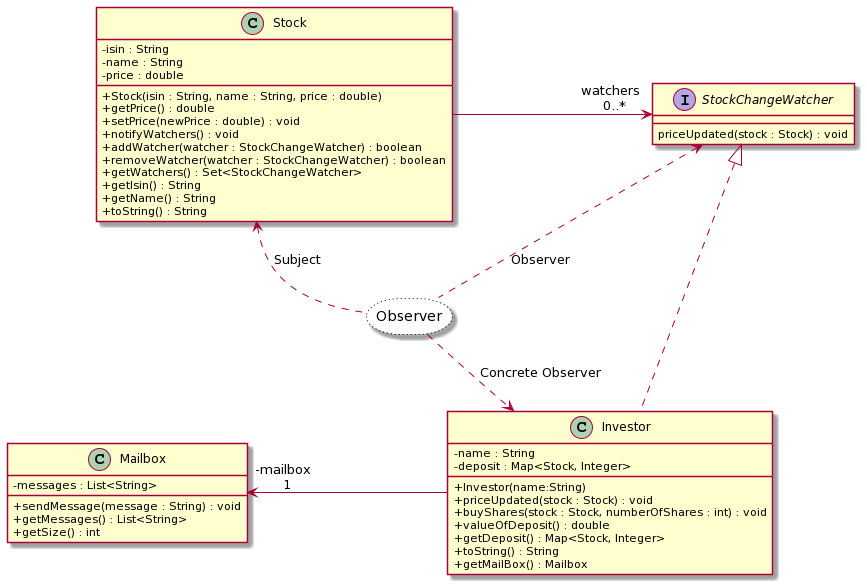
\includegraphics[width=0.75\textwidth]{./Aufgabe8_1}
		\end{center}
	\end{enumerate}

	\section*{Aufgabe 2}
	\begin{lstlisting}[style=java,tabsize=2]
/**
* Aktien werden durch eine feste ISIN (International Securities Identification
* Number) und einen festen Namen beschrieben und koennen ihren Preis aendern.
* Durch einen Benachrichtigungsmechanismus ({@link StockChangeWatcher}) koennen
* interessierte Parteien ueber Preisverfaelle informiert werden.
*/
public class Stock {
	private final String isin;
	private final String name;
	private double price;
	private double oldPrice;

	private final Set<StockChangeWatcher> watchers = new HashSet<>();

	public Stock(String isin, String name, double price) {
		this.isin = isin;
		this.name = name;
		this.price = price;
		this.oldPrice = price;
	}

	public double getPrice() {
		return price;
	}

	public void setPrice(double newPrice) {
		if (newPrice < 0.0) {
			throw new IllegalArgumentException("newPrice darf nicht negativ sein");
		} else {
			this.oldPrice = price;
			this.price = newPrice;
			notifyWatchers();
		}
	}

	private void notifyWatchers() {
		for (StockChangeWatcher w : watchers) {
			// Preisaenderung negativ
			if (price < oldPrice) {
				w.priceUpdated(this);   
			}
		}
	}

	public boolean addWatcher(StockChangeWatcher watcher) {
		return watchers.add(watcher);
	}

	public boolean removeWatcher(StockChangeWatcher watcher) {
		return watchers.remove(watcher);
	}

	public Set<StockChangeWatcher> getWatchers() {
		return Collections.unmodifiableSet(watchers);
	}

	public String getIsin() {
		return isin;
	}

	public String getName() {
		return name;
	}

	public String toString() {
		return name + " (" + isin + ")";
	}
}
	\end{lstlisting}

	\section*{Aufgabe 3}
	\begin{enumerate}[label=(\alph*)]
		\item Testfalltabelle
		\begin{center}
			\begin{tabular}{c|C{5cm}|c|C{5cm}}
				\textbf{Testfall} & \textbf{Aufruf} & \textbf{Eingabe} & \textbf{Erwartetes Ergebnis} \\
				\hline
				ON1 & stock.setPrice & 0.0 & investor wird benachrichtigt \\
				\hline
				ON2 & stock.setPrice & -1.0 & IllegalArgumentException wird in stock geworfen, investor wird nicht benachrichtigt \\
				\hline
				ON3 & stock.setPrice & 500 & investor wird nicht benachrichtigt \\
				\hline
				ON4 & stock.setPrice & 15.37 & investor wird nicht benachrichtigt \\
				\hline
				ON5 & stock.removeWatcher(investor); stock.setPrice & 10 & investor wird nicht benachrichtigt \\
				\hline
				ON6 & stock.setPrice & 10 & investor wird benachrichtigt
			\end{tabular}
		\end{center}
		\item Implementierung
		\begin{lstlisting}[style=java, tabsize=2]
import static org.junit.jupiter.api.Assertions.*;
import org.junit.jupiter.api.*;

/**
* Testet die Interaktion von {@link Stock}- und {@link Investor}-Objekten (Test
* von Objektnetzen).
*/
class ChangeNotificationTest {
	private Investor investor;
	private Mailbox mailbox;
	private Stock stock;


	@BeforeEach
	void setUp() {
		investor = new Investor("Erika Musterfrau");
		mailbox = investor.getMailbox();
		stock = new Stock("US36467W1099", "GME", 15.37);
		stock.addWatcher(investor);
	}

	@Test
	void Test1() {
		stock.setPrice(0.0);
		assertEquals(1, mailbox.getSize());
		assertEquals("Neuer Wert von GME (US36467W1099): $0.0", mailbox.getMessages().get(0));
	}

	@Test
	void Test2() {
		try {
			stock.setPrice(-1.0);
			fail("setPrice() sollte keine negativen Werte akzeptieren");
		} catch (IllegalArgumentException e) {
			System.out.println("GG");
		}
		assertEquals(0, mailbox.getSize());
	}

	@Test
	void Test3() {
		stock.setPrice(500.0);
		assertEquals(0, mailbox.getSize());
	}

	@Test
	void Test4() {
		stock.setPrice(15.37);
		assertEquals(0, mailbox.getSize());
	}

	@Test
	void Test5() {
		stock.removeWatcher(investor);
		stock.setPrice(10.0);
		assertEquals(0, mailbox.getSize());
	}

	@Test
	void Test6() {
		stock.setPrice(10.0);
		assertEquals(1, mailbox.getSize());
	}
}
		\end{lstlisting}
		Ablauf Testfall ON6
		\begin{center}
			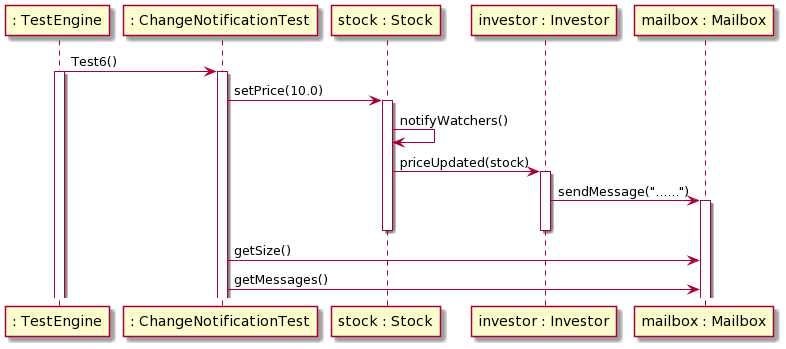
\includegraphics[width=0.75\textwidth]{./Aufgabe8_3}
		\end{center}
	\end{enumerate}
\end{document}